%analysis and solution: mathematics/algorithms/system design

\subsection{Data structures}

We call the final generated terrain a \textbf{Map}.
A Map is a collection of \textbf{Center}s, \textbf{Corner}s and \textbf{Edge}s.

\paragraph{Center} has the following properties:

\begin{itemize}
	\item Vec2 point
	\item bool water
	\item bool ocean
	\item bool coast
	\item bool border
	\item float elevation
	\item float moisture
	\item Biome biome
	\item Center[] neighbours
	\item Edge[] borders
	\item Corner[] corners
\end{itemize}

\paragraph{Corner} has the following properties:

\begin{itemize}
	\item Vec2 point
	\item bool water
	\item bool ocean
	\item bool coast
	\item bool border
	\item float elevation
	\item float moisture
	\item int river
	\item int watershed\_size
	\item Corner downslope
	\item Corner watershed
	\item Center[] touches
	\item Edge[] protrudes
	\item Corner[] adjacent
\end{itemize}

\paragraph{Edge} has the following properties:

\begin{itemize}
	\item Center delaunay0
	\item Center delaunay1
	\item Corner voronoi0
	\item Corner voronoi1
	\item int river
	\item Vec2 midway\_point
\end{itemize}

\subsection{Generation}

The terrain generation happens in the following stages:

\begin{enumerate}
	\item Placing points
	\item Building graph
	\item Shaping island
	\item Assigning elevations
	\item Assigning moisture and rivers
	\item Assigning biomes
\end{enumerate}

\paragraph{Placing points}

In this stage, the points that make up the center of the polygons are selected.
We currently have a selector that returns random points, one that uses poisson trials for better randomness, one that returns points that result in a hexagonal voronoi diagram and one that results in a grid-like voronoi diagram.

The selected points become the centers of the map.

Figure~\ref{fig:algo:points} shows an example of selected points.

Algorithm~\ref{alg:point} gives pseudo-code for the point selector that results in a grid-like structure.

\begin{algo*}
\begin{sourcecode}
\algorithm{SquarePointSelector($width, height, n$)}
$P = \emptyset$
\for{$i = 0; i < \sqrt{n}; i++$}
	\for{$i = 0; i < \sqrt{n}; i++$}
		$P = P \cup \left<\frac{0.5 + i}{n} width, \frac{0.5 + j}{n} height\right>$
	|
|
\return P
\qend
\end{sourcecode}
	\caption{Point selection algorithm}
	\label{alg:point}
\end{algo*}

\paragraph{Building graph}

Next, we use the selected points to build the data structures that represent the map.
We do this by constructing a Voronoi diagram (using Fortune's algorithm) and a Delaunay triangulation and creating polygons from that.

All nodes in the Voronoi diagram become corners, all edges in the Voronoi diagram, together with their dual edge in the Delaunay triangulation, are saved as edges in the map.

Figure~\ref{fig:algo:voronoi} shows an example of a generated Voronoi diagram, Figure~\ref{fig:algo:delaunay} gives the resulting Delaunay triangulation.

\paragraph{Shaping island}

The island shape is a function that determines which of the centers in the map are part of the island and which are water.

In Figure~\ref{fig:algo:polygons}, an example island shape is shown.

\paragraph{Assigning elevations}

In the elevations step, we first assign elevations to corners by going from the ocean inwards, increasing the elevation by 1 whenever we move to a new rank.
Then, we redistribute the elevations by sorting all corners on elevation, and evenly distributing elevations from 0 to 1 among them.
Finally, we set the elevation of each center to the average of its corners.

Figure~\ref{fig:algo:elevation} gives an example of elevations.

\paragraph{Assigning moisture and rivers}

First, we calculate the corner that is downslope for each corner in the map.
Then, we use this to calculate watersheds.
After that, we randomly select a number of springs on the map, where we start a river.
From each spring, we follow the watershed corners until we reach the ocean.

Then, we assign moisture to each corner based on the distance to a river or a body of water and we redistribute moisture like elevation.
Finally, we set the moisture of each center to the average of its corners.

\paragraph{Assigning biomes}

Finally, we use the moisture and elevation properties of each center to assign a biome.

\begin{figure}
	\centering
	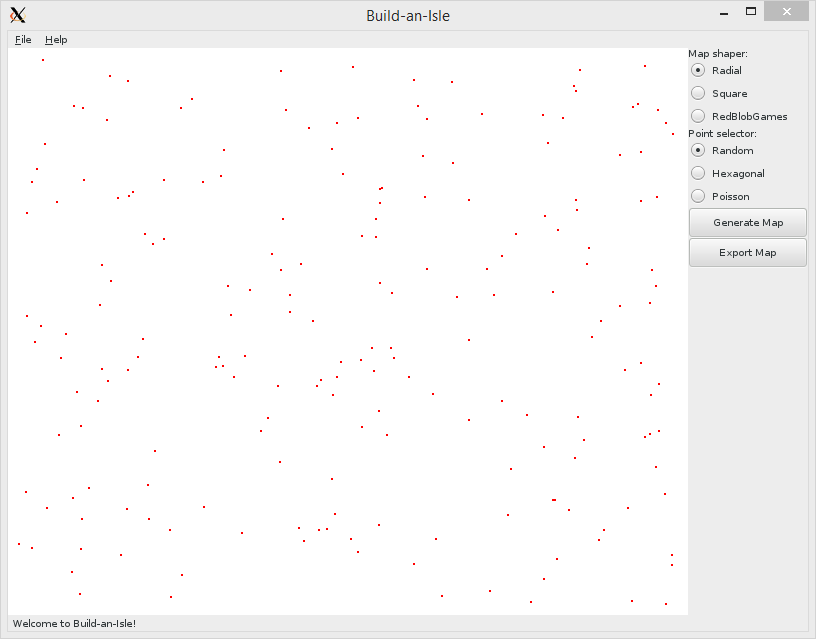
\includegraphics[width=0.8\linewidth]{points}
	\caption{Selecting points}
	\label{fig:algo:points}
\end{figure}

\begin{figure}
	\centering
	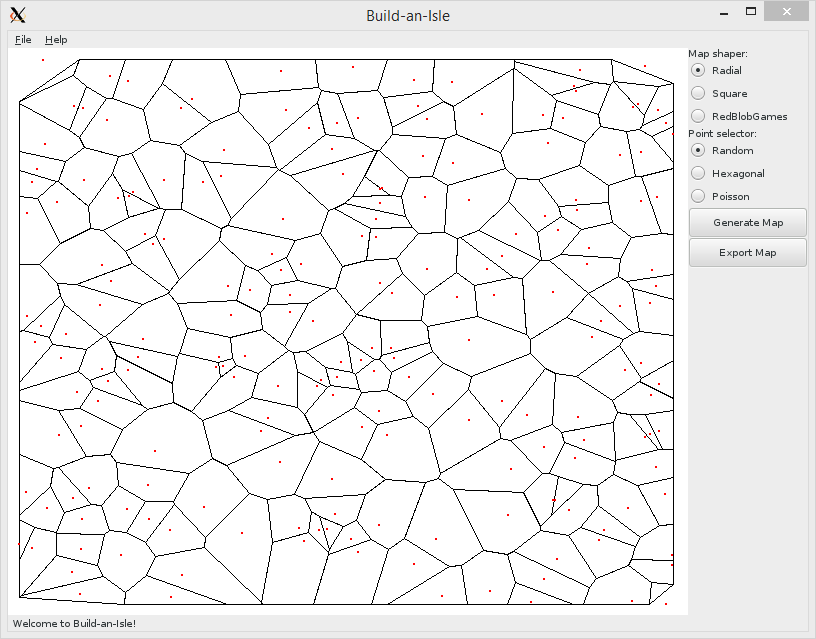
\includegraphics[width=0.8\linewidth]{voronoi}
	\caption{Building a Voronoi diagram}
	\label{fig:algo:voronoi}
\end{figure}

\begin{figure}
	\centering
	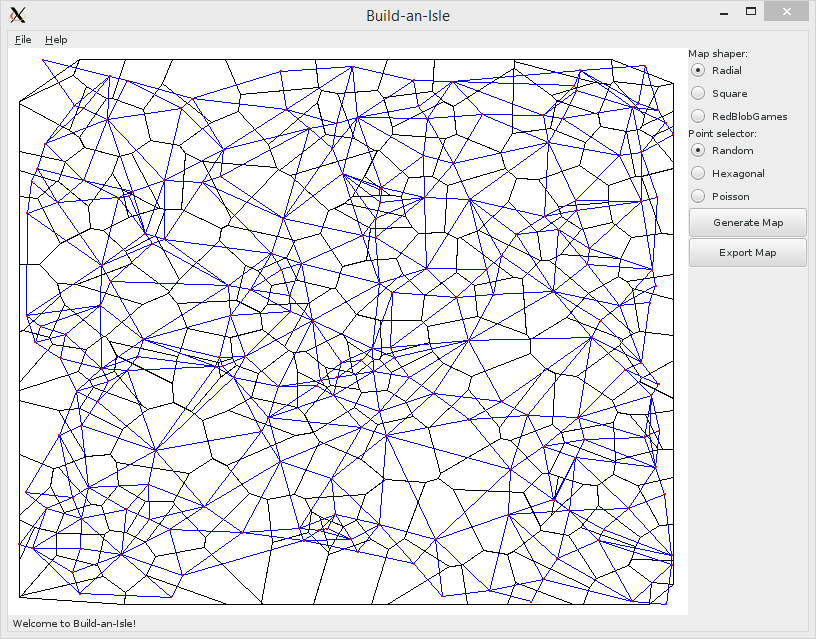
\includegraphics[width=0.8\linewidth]{delaunay}
	\caption{Delaunay triangulation}
	\label{fig:algo:delaunay}
\end{figure}

\begin{figure}
	\centering
	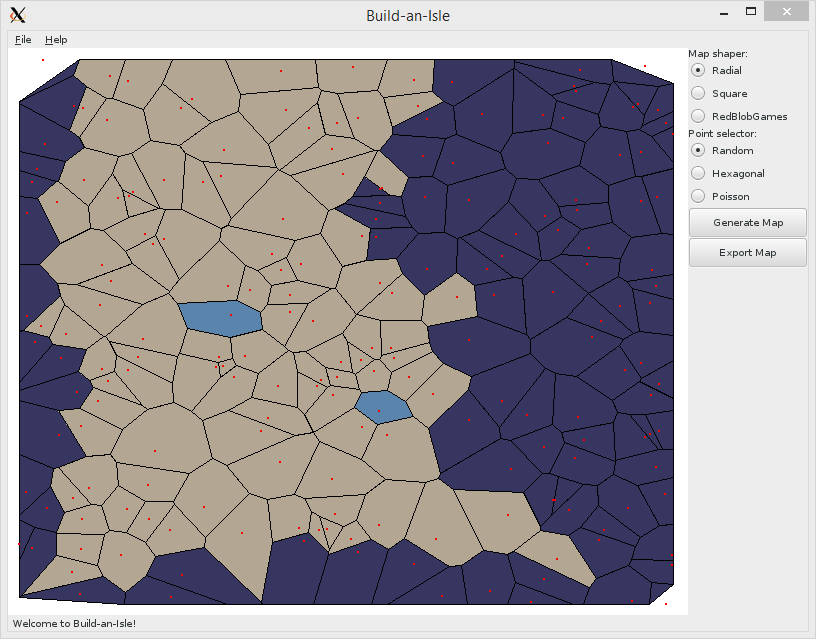
\includegraphics[width=0.8\linewidth]{polygons}
	\caption{Determining island shape}
	\label{fig:algo:polygons}
\end{figure}

\begin{figure}
	\centering
	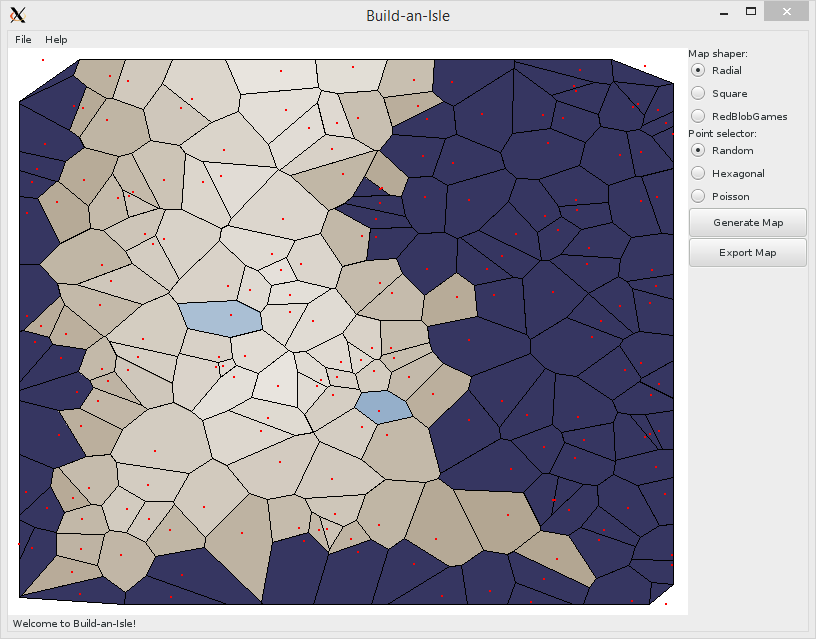
\includegraphics[width=0.8\linewidth]{elevation}
	\caption{Setting elevation}
	\label{fig:algo:elevation}
\end{figure}

%TODO: Similar images for the next steps

\subsection{System design}

Using wxWidgets we set up a window with the necessary controls to modify parameters with which to generate maps and export them. Within this window we will be using OpenGL to visualize the generation process and provide the user with an idea of what the map might look like in the viewer application.

\subsubsection{Preview rendering}

We want to give the user a good idea of what is being generated and how this is being done. This will highlight the workings of the generation process and allow the user to intuitively judge wether he or she should adjust the parameters.

\paragraph{Shaders}

Whenever we will be rendering anything we will be using appropriate shaders. For now we will be using a pair of relatively simple vertex and fragment shaders to be extended where needed. To start with they take into account the projection, position of the camera and model matrix for whichever object is being drawn. Furthermore each vertex has an associated position, normal and color. These are more or less minimal requirements to render anything. They also consider a single light source to add some dynamics to the map preview. 

Even with these simple shaders we can observe the effect of the calculations of the fragment shader in that eventual lighting dependent output colours are determined not per vertex but per pixel. This is one of the more obvious advantages of using our custom shaders.
